%%%%%%%%%%%%%%%%%%%%%%%%
%
% $Author: Chung Man Tsang$
% $Datum: 2024-05-21  $
% $Pfad: BATime-Series/report/Contents/en/Kerass.tex $
% $Version: 1.0 $
% $Reviewed by: Chung Man Tsang  $
% $Review Date: 2024-05-21 $
%
% $Short Description: Explanation about Keras $
%%%%%%%%%%%%%%%%%%%%%%%%


\chapter{Keras Package}
\section{Introduction}
Keras is an open-source high-level, deep learning API produced by Google for neural network implementation. It can run on top of TensorFlow, PyTorch and JAX . Keras offers 'simple', 'flexible', and 'powerful' features for implementing neural network function in Python.\cite{kerasteam:2024}. 
Therefore, based on the three features Keras described, it was primarily developed for rapid experimentation and prototype designing with Keras. You can create your deep learning architecture using a few lines of code. Moreover, Keras provides a high level of abstraction for developing and shipping of machine learning applications. You can create almost all popular deep learning architectures by calling the APIs without even implementing
the complex underlying functionalities. Keras comes as a high- level set of APIs directly integrated with TensorFlow, which can be directly called from TensorFlow. It enables you to exploit the full advantage of the scalability and cross-platform
capabilities of TensorFlow. Hence, Keras can be run on GPU, TPU and CPU without any barriers, given the framework used.\cite{Kerasteam:2024} \\

Moreover, Keras APIs can be directly integrated with TensorFlow. While Keras started as a standalone library to simplify building neural networks, it is integrated as a part of Tensorflow and can utilize it as "tf.keras". \cite{keras:2023}


\section{Description}
As a fast recap, Keras is a high-level neural networks API, written in Python and capable of running on top of TensorFlow, Theano, or Microsoft Cognitive Toolkit (CNTK).\cite{simplilearn:2024} It focuses on enabling fast experimentation and easy prototyping of deep learning models. Keras provides a user-friendly interface that allows for the construction, training, and deployment of neural networks with minimal code.\\

The Keras package has 5 main components:
\begin{itemize}
	\item \textbf{Model}: The central abstraction in Keras is the model. The primary model type is the \textbf{Sequential} model, a linear stack of layers, which is straightforward and widely used for many deep learning applications. Alternatively, the Functional API allows for more complex architectures, enabling models that have non-linear topology, shared layers, and multiple inputs or outputs.
	\item \textbf{Layers}: Layers are the fundamental building blocks of neural networks in Keras. Keras provides a wide range of pre-built layers, such as dense (fully connected) layers, convolutional layers, pooling layers, and recurrent layers (including LSTMs). Custom layers can also be created, offering flexibility to implement proprietary algorithms.
	\item \textbf{Compilers}: Once a model is defined, it needs to be compiled. This step involves specifying the loss function and the optimizer. Keras provides numerous choices for both, including pre-defined loss functions like categorical\_crossentropy or mse and optimizers like Adam, SGD, or RMSprop.
	\item \textbf{Training}: Training a model in Keras involves calling the fit method, passing in the training data, specifying the number of epochs, and, optionally, the batch size. Keras also supports callbacks during training that allow for actions at various stages of the training cycle, such as model checkpointing, learning rate adjustments, and early stopping.
	\item \textbf{Evaluation and Prediction}: After training, models can be evaluated using the evaluate method, which requires test data. Predictions can be made using the predict method.
\end{itemize}

Overall, we firstly configure our model for training by specifying the loss function, optimizer, and evaluation metric. Since we are dealing with a multi-class classifier problem, we will use a loss function readily available in Keras, the categorical cross-entropy loss function. We will use Adam as an optimizer to minimize the loss, which is a very popular choice in deep neural networks owing to its adaptive learning rate. We will use the default learning rate. Finally, we provide classification accuracy as a metric to judge our model's performance during training. The function \texttt{model.compile()} is used to configure the process. Refer to the following code:

\begin{lstlisting}[language=Python]
	
model.compile(loss='categorical_crossentropy',
optimizer='adam', metrics=['accuracy'])
\end{lstlisting}


Then, we are ready to train our model. We will call the function \texttt{model.fit()}. The training data and the labels are supplied as input parameters. We also specify two more hyperparameters, the mini-batch size, and the number of epochs for training. The mini-batch size specifies how much of the data is used to compute the loss function and update the weights in one iteration.

The ideal case for the model can give around 95\% classification accuracy on the training data. Next, we need to see how the model performs on the untrained data. We will call the function \texttt{model.evaluate()}. 

\section{Installation}
	
To install Keras for our project, we have to typically work with Keras within a Python environment on our development machine. Here's how you can install Keras:

\begin{enumerate}
	\item \textbf{Python Installation}: Make sure you have Python installed on your system. You can download and install Python from the official website: Python.org. The detailed explanation on Python Installation is on the software description.\ref{Python}
	
	\item \textbf{Package Manager}: Python has the default package manager called \textbf{pip}, which can install Python packages, including Keras. 
	
	\item \textbf{\ac{ide}}: As we use the Pycharm \ref{Pycharm} for the python environment, we can also install the package through the function of pycharm with several clicks to install the package. 

	
\end{enumerate}

\subsection{Install Keras via pip}

Open your terminal or default command prompt and run the following command when you open the python environment:

\begin{lstlisting}[language=Python]
	
		pip install keras 
	
	
\end{lstlisting}

This will download and install the latest version of Keras along with its dependencies.

\subsection{Install Keras via Pycharm}
Keras can be installed through the Pycharm IDE. We can follow the following procedure simply with several clicks. Here is the procedures that we can install:

\begin{enumerate}
	\item Click the Python Package Button at the left-side bar
	\begin{figure}[h!]
		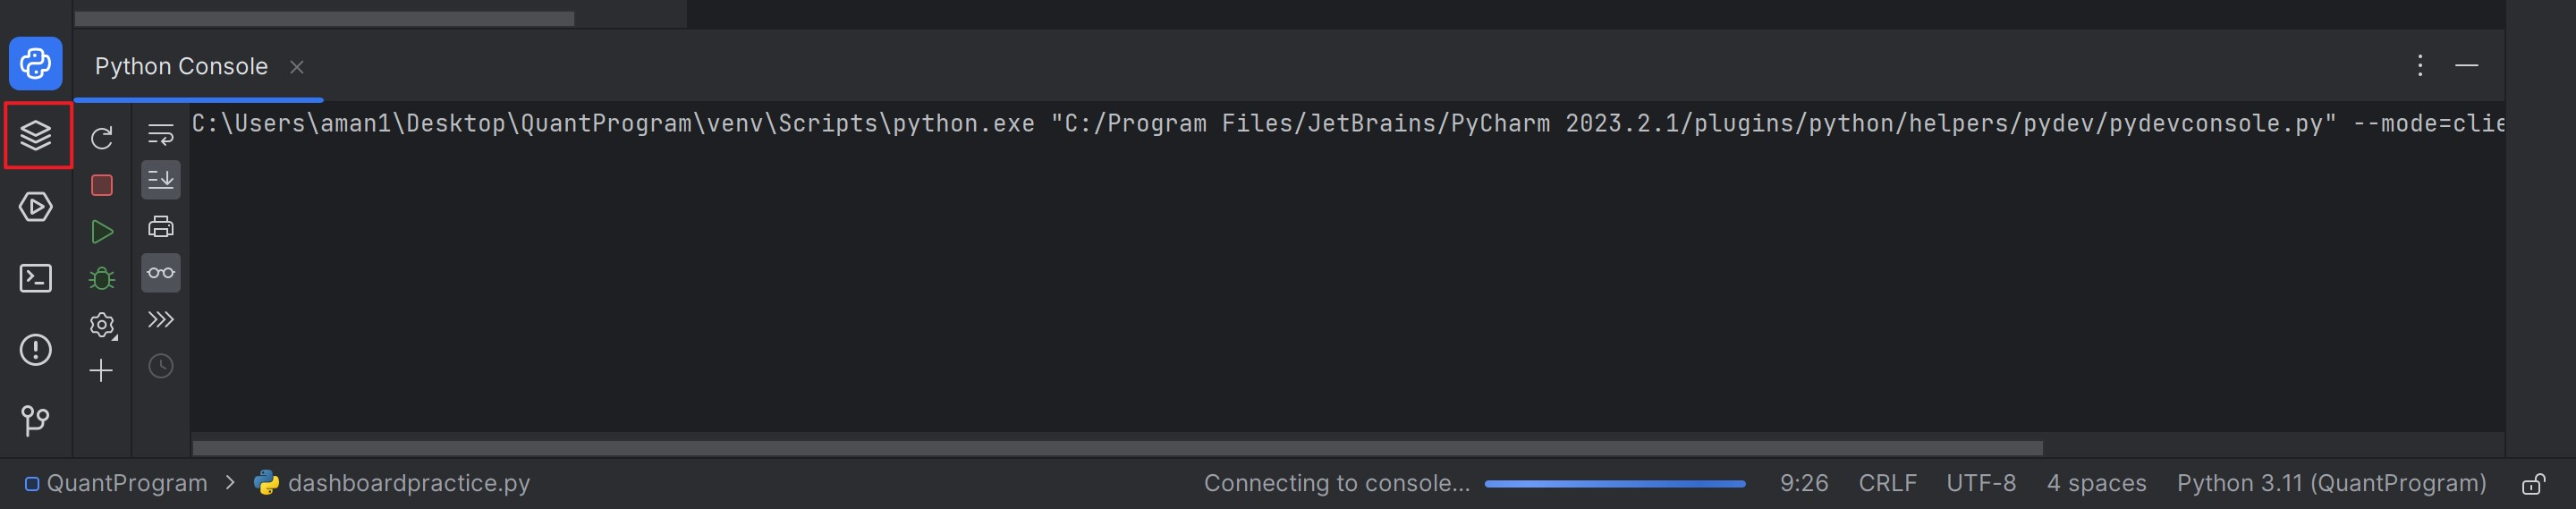
\includegraphics[width=\textwidth]{Images/Keras/PackagePycharmStep1}
		\caption{Install Package at Pycharm Step 1}
	\end{figure}
	\item Type the package that we would like to install
	\begin{figure}[h!]
		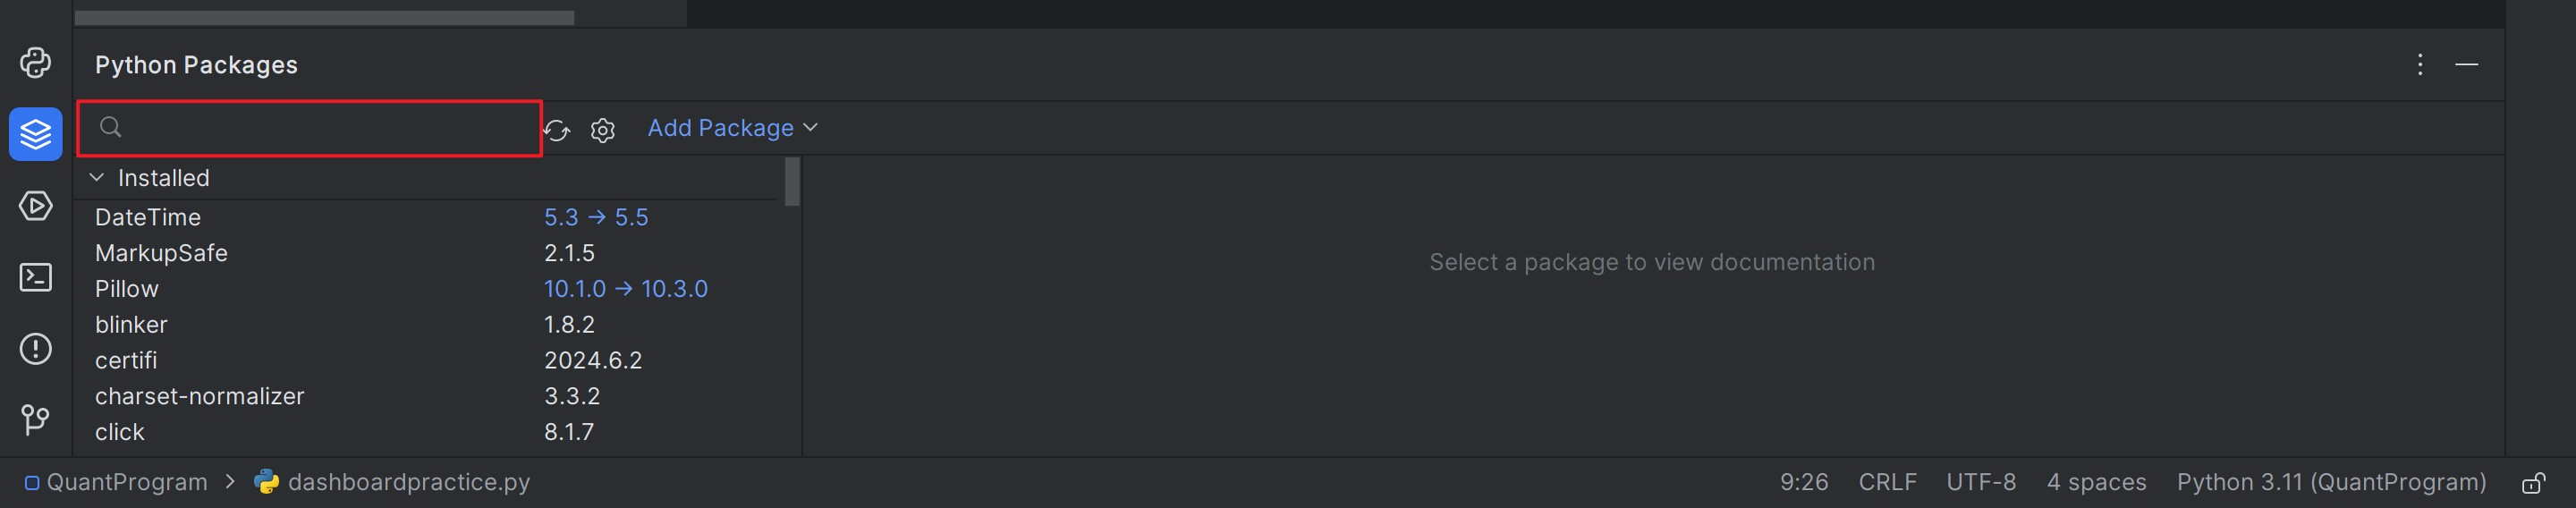
\includegraphics[width=\textwidth]{Images/Keras/PackagePycharmStep2}
		\caption{Install Package at Pycharm Step 2}
	\end{figure}
	\item Click the install button and select the version that is required to download
	\begin{figure}[h!]
		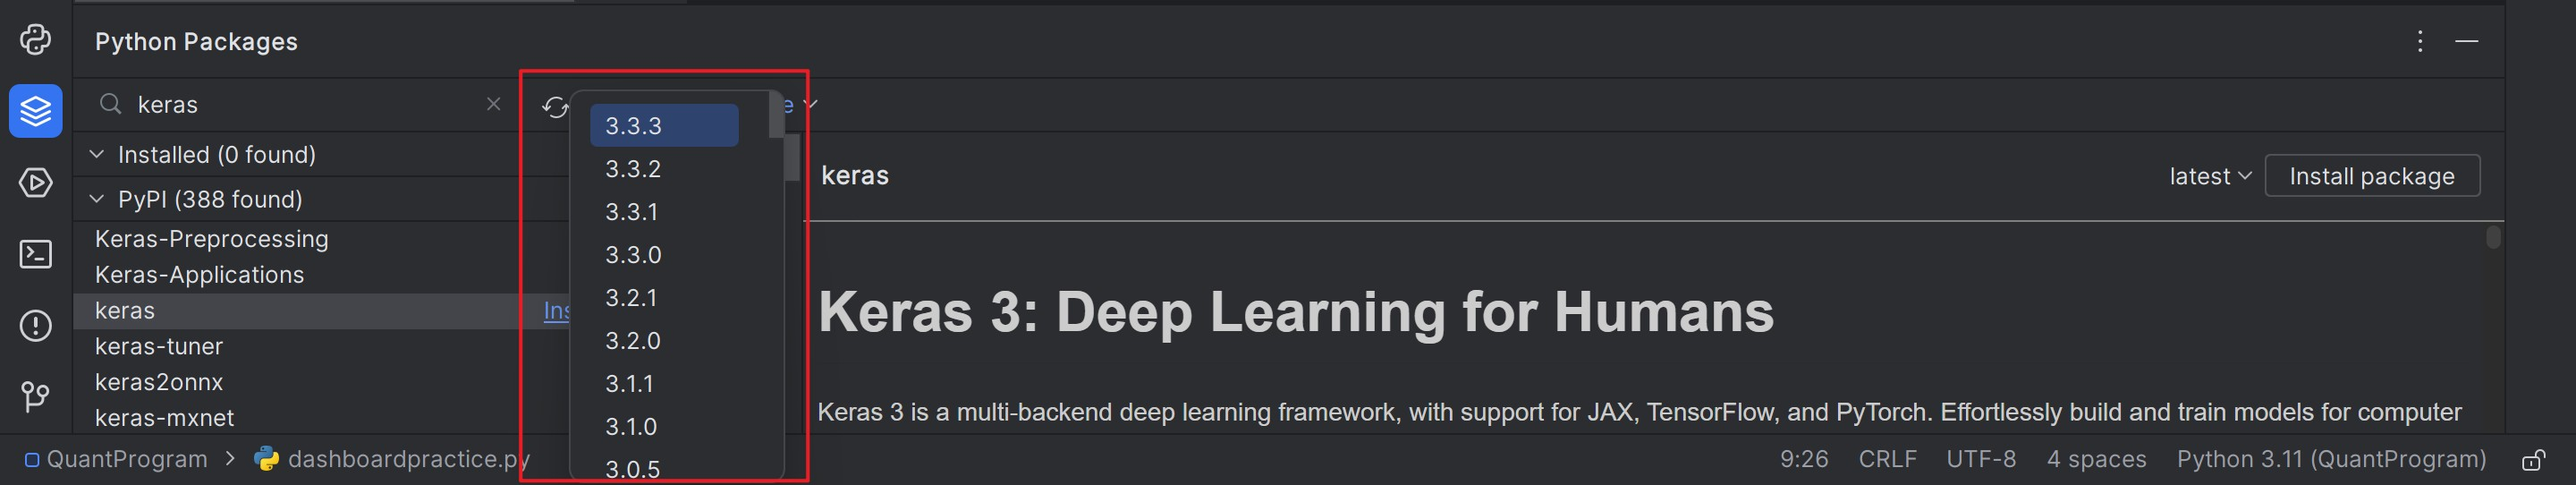
\includegraphics[width=\textwidth]{Images/Keras/PackagePycharmStep3}
		\caption{Install Package at Pycharm Step 3}
	\end{figure}
	\item After installation, you can see your implemented package in the installed region
	\begin{figure}[h!]
		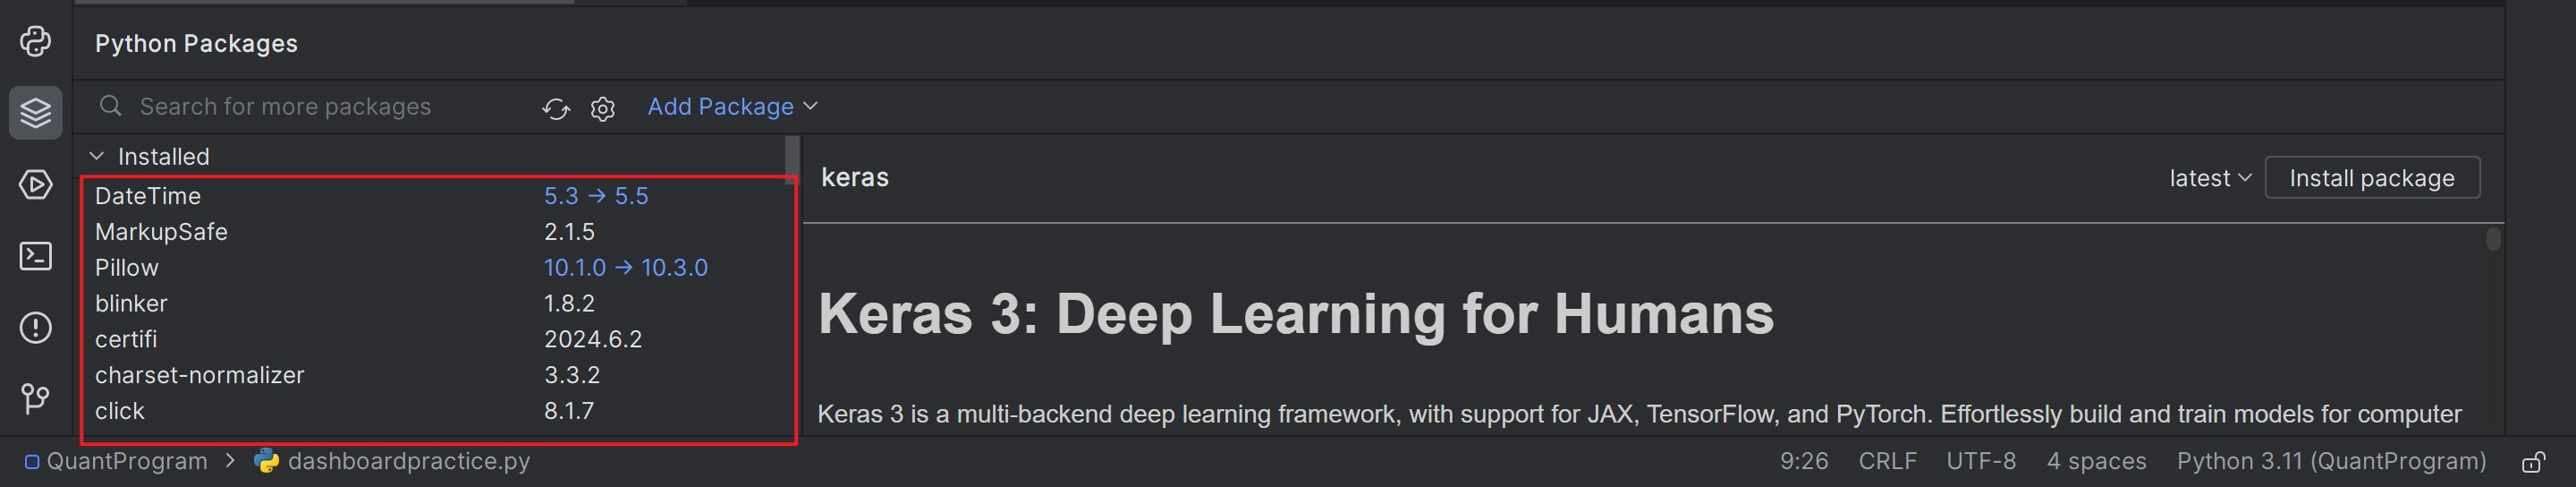
\includegraphics[width=\textwidth]{Images/Keras/PackagePycharmStep4}
		\caption{Install Package at Pycharm Step 4}
	\end{figure}
\end{enumerate}

\subsection{Install Keras with TensorFlow backend}

Keras can also be installed as part of the TensorFlow package, which includes Keras as its high-level API. If you're planning to use TensorFlow as the backend for Keras, you can install TensorFlow instead, and Keras will be automatically included. In the \\To install TensorFlow with Keras, run:

\begin{lstlisting}[language=Python]
	
	pip install tensorflow
	
	
\end{lstlisting}


\subsection{Checking the Installation}

After installation, you can verify that Keras is installed correctly by opening a Python interpreter and importing Keras:

\begin{lstlisting}[language=Python]
	
	import keras
	print(keras.__version__)
	
	
\end{lstlisting}
This should print the version of Keras installed on your system.\cite{Keinstall:2024}

\subsubsection{Note}

\begin{enumerate}
	\item Ensure that your Python environment is properly configured with the necessary libraries
	
	\item If you're planning to train deep learning models on your development machine, make sure your machine meets the hardware and software requirements for running Keras and TensorFlow efficiently.
	
\end{enumerate}

	\subsection{updating the version of Keras in Python}

To update the version of Keras in Python, you can use the pip package manager. Here are the steps:


\begin{enumerate}
	\item Open your command line or terminal.
	\item Run the following command:
	
	
	
	\begin{lstlisting}[language=python]
		pip install --upgrade keras
	\end{lstlisting}
	
	
	This command will upgrade the Keras package to the latest version available on the Python Package Index (PyPI).
	
	\item Once the upgrade is complete, you can verify the updated version by running:
	
	\begin{lstlisting}[language=python]
		python -c "import keras; print(keras.__version__)"
	\end{lstlisting}
	
	
	This command will print out the version of Keras installed in your Python environment, confirming that the update was successful.
\end{enumerate}

By following these steps, you can ensure that you have the latest version of Keras installed.\cite{Lak:2023}


\section{Example - Description}

	In our project, Keras can be used to implement machine learning algorithms for gesture recognition. Below is an example code description demonstrating how Keras can be used:
	\begin{lstlisting}[language=Python]

	import keras
	from keras.models import Sequential
	from keras.layers import Conv2D, MaxPooling2D, 
	Flatten, Dense
	
	# Define the architecture of the neural network
	model = Sequential()
	model.add(Conv2D(32, kernel_size=(3, 3), 
	activation='relu', input_shape=(28, 28, 1)))
	model.add(MaxPooling2D(pool_size=(2, 2)))
	model.add(Flatten())
	model.add(Dense(128, activation='relu'))
	model.add(Dense(10, activation='softmax'))
	
	# Compile the model
	model.compile(optimizer='adam', 
	loss='sparse_categorical_crossentropy', metrics=['accuracy'])
	
	# Train the model
	model.fit(train_images, train_labels, epochs=10,
	validation_data=(test_images, test_labels))
	
	# Evaluate the model
	test_loss, test_acc = 
	model.evaluate(test_images, test_labels)
	print('Test accuracy:', test_acc)

	\end{lstlisting}
This example code demonstrates a typical usage of Keras for building, training, and evaluating a neural network model for gesture recognition. Adjust the model architecture, training parameters, and evaluation metrics as needed for your specific project requirements.

By leveraging Keras for the business analytics project, our team can create the training model with Keras easily as the feature of ease of use of it.\\Keras contains numerous implementations of commonly used neural-network building blocks such as layers, objectives, activation functions, optimizers, and a host of tools for working with image and text data to simplify programming in the deep neural network area.

Furthermore, Keras 3, as the latest version as of the package, supports multiple backends including TensorFlow, JAX, and PyTorch1. It can now run your high-level Keras workflows on top of any of these frameworks, benefiting from the advantages of each. We can import the keras class directly like "tensorflow.keras.models" even we only use the tensorflow package. 

	\section{Example - Manual}

	\subsection{Introduction to Keras}
	Keras is a high-level neural networks API written in Python. It's designed to be user-friendly, modular, and extensible, allowing for easy experimentation and prototyping of deep learning models. In the context of business data analytics , Keras can be a powerful tool for implementing machine learning algorithms for gesture recognition.\cite{Keras:2023}

	\subsection{Procedures}
	\subsubsection{Installation}
	
	
	\begin{lstlisting}[language=bash]
pip install tensorflow	
	\end{lstlisting}

	\subsubsection{Getting Started}
	Once tensorflow is installed, you can import it in your Python scripts or interactive sessions:
	
	\begin{lstlisting}[language=python]
import pandas as pd
import tensorflow as tf
from tensorflow.keras.models import Sequential
from tensorflow.keras.layers import Dense
	
	\end{lstlisting}

	\subsubsection{Create the own dataset or load the dataset}
Normally, based on the condition of project, we may have the own data source or use the data from the external to create the dataset. At this point, we also need to load the dataset in the script so that we can further develop the data model. \cite{brownlee:2022}

\begin{lstlisting}[language=python]
	
#read the data and check the data content 
data = pd.read_csv("data.csv")
print(data.head(), data.columns)

# split into input (X) and output (y) variables
X = data[:,0:8]
y = data[:,8]

\end{lstlisting}

\subsubsection{Define a Sequential Model}

Keras provides a Sequential model API for building neural networks layer-by-layer. Here's an example of how to create a simple Sequential model with Keras:

	\begin{lstlisting}[language=python]

# Initialize the model
model = Sequential()

# Add layers to the model
model.add(Dense(12, input_shape=(8,), activation='relu'))
model.add(Dense(8, activation='relu'))
model.add(Dense(1, activation='sigmoid'))

\end{lstlisting}

\subsubsection{Compile a Sequential Model}

Compile the model with an optimizer, a loss function, and a metric to monitor:

\begin{lstlisting}[language=python]
	
model.compile(loss='binary_crossentropy', optimizer='adam',
metrics=['accuracy'])

\end{lstlisting}

\subsubsection{Training the Model}

Once the model is defined, you can train it on your data. Here's an example of how to train the model:
	
	\begin{lstlisting}[language=python]
	
# Assuming X and y are your training data
model.fit(X, y, epochs=150, batch_size=10)

\end{lstlisting}

\subsubsection{Evaluating the Model}

After training, you can evaluate the performance of the model on your test data:

	\begin{lstlisting}[language=python]
	
# Assuming X and y are your test data and evaluate it
_, accuracy = model.evaluate(X, y)
print('Accuracy: \%.2f' \% (accuracy*100))

	
\end{lstlisting}

For a detailed guide covering in-depth usage of different parts of the Keras API, you can refer to the Keras developer guides. These guides are deep-dives into specific topics such as layer subclassing, fine-tuning, or model saving.\cite{Keinstall:2024}

\subsection{Important attributes of keras}

	\begin{enumerate}
		\item \textbf{Simplicity}: Keras is designed to be simple and easy to use. It provides a high-level interface that abstracts away many complexities of building neural networks, making it accessible to beginners and experts alike.
		
		\item \textbf{Modularity}: Keras allows for easy construction of complex neural network architectures through a modular approach. Neural network models are built by stacking layers on top of each other, and each layer can be easily added, removed, or modified.
		
		\item \textbf{Flexibility}: Keras supports both sequential and functional API for building models. The sequential API is used for simple linear stacks of layers, while the functional API allows for more complex architectures with shared layers, multiple inputs, and multiple outputs.\cite{Attrik:2020}
		
		\item \textbf{Compatibility}: Keras is compatible with multiple backend engines, including TensorFlow, Theano, and Microsoft Cognitive Toolkit (CNTK). This allows users to choose the backend that best suits their needs.
		
		\item \textbf{Customization}: Keras provides a wide range of built-in layers, loss functions, optimizers, and metrics. Additionally, users can easily define custom layers, loss functions, and metrics to meet specific requirements.
		
		\item \textbf{Integration}: Keras seamlessly integrates with other popular Python libraries and frameworks, such as TensorFlow and scikit-learn. This allows for easy interoperability and integration into existing workflows and projects.
		
		\item \textbf{Community and Documentation}: Keras has a large and active community of developers and users who contribute to its development and provide support. The official documentation is comprehensive and includes tutorials, guides, and API references to help users get started and learn more about Keras.
	\end{enumerate}
	
	These attributes make Keras a powerful and versatile tool for building and training neural networks for a wide range of applications. For instance, our project can rely on the keras package to build the LSTM data model.

\subsection{Example - Code}
	
	After the discussion of the manual, we clearly defined that keras package theoretically involves 5 core components. These 5 components turn out to various steps needed to follow from the scratch to the evaluation and prediction phase. The completed code example would be shown here. 
	
	\begin{lstlisting}[language=python]
		
import tensorflow as tf
from tensorflow.keras.models import Sequential
from tensorflow.keras.layers import Dense
from sklearn.model_selection import train_test_split
from sklearn.datasets import make_circles
import numpy as np

# Generate synthetic data
X, y = make_circles(n_samples=1000, factor=0.5,
noise=0.05, random_state=42)

# Split the data
X_train, X_test, y_train, y_test = train_test_split
(X, y, test_size=0.3, random_state=42)

# Build the model
model = Sequential([
Dense(10, activation='relu', input_shape=(2,)),
Dense(10, activation='relu'),
Dense(1, activation='sigmoid')
])

# Compile the model
model.compile(optimizer='adam',
loss='binary_crossentropy',
metrics=['accuracy'])

# Train the model
history = model.fit(X_train, y_train, epochs=50,
batch_size=10, validation_split=0.2)

# Evaluate the model
loss, accuracy = model.evaluate(X_test, y_test)
print("Test accuracy:", accuracy)

# Predict new data
new_data = np.array([[0.1, 0.0], [1.2, 1.0]])
predictions = model.predict(new_data)
print("Predictions:", predictions.squeeze())
		
		
	\end{lstlisting}


This example code demonstrates how to build, compile, train, and evaluate a simple neural network model using Keras for the project. Adjust the architecture, hyperparameters, and preprocessing steps as needed to fit your specific requirements and dataset.


	\section{Example - Files}
Given Keras main function for developing the neural network, keras also provides some file operations functions to fulfill the need for users loading and saving models. To further handle the data files in other formats such as jpeg, jpg, we can also collaborate the functions in tensorflow to further support\ref{handlefileswithtensorflow}. First of all, focusing only on Keras, it can perform the saving functions through the following code execution in the script:

\begin{enumerate}
	\item \textbf{Loading and Saving Models}: Keras allows you to save the entire model, including its architecture, weights, and training configuration, in a single file. You can also choose to save only the architecture or only the weights.
	\begin{lstlisting}[language=python]
	#Saving the Entire Model
	# Saves as a TensorFlow SavedModel
	model.save('my_model')     
	
	#Load a Saved Model
	from tensorflow.keras.models import load_model
	
	# Load a model
	# Load from HDF5
	model = load_model('my_model.h5')
	# Load from SavedModel  
	model = load_model('my_model')   
	
	#Saving Weights
	model.save_weights('my_model_weights.h5')
	
	# Loading Weights
	model.load_weights('my_model_weights.h5')
	
	\end{lstlisting}
\end{enumerate}

	\subsection{Example for loading image files}\label{handlefileswithtensorflow}
	
		\begin{lstlisting}[language=python]
		
import numpy as np
from keras.models import Sequential
from keras.layers import Dense, Flatten, Conv1D, MaxPooling1D
from keras.optimizers import Adam
	
import tensorflow as tf

def parse_function(filename, label):
image_string = tf.io.read_file(filename)
image_decoded = tf.image.decode_jpeg(image_string, channels=3)
image_resized = tf.image.resize(image_decoded, [224, 224])
return image_resized, label

def create_dataset(filenames, labels):
dataset = tf.data.Dataset.from_tensor_slices((filenames, labels))
dataset = dataset.map(parse_function)
return dataset

# Assuming you have a list of image paths and corresponding labels
filenames = ['path/to/image1.jpg', 'path/to/image2.jpg']
labels = [0, 1]  # example labels

dataset = create_dataset(filenames, labels)
for image, label in dataset.take(2):
print(image.shape, label)
	\end{lstlisting}
	
	This script demonstrates how to load images, decode them, resize them, and prepare them for model training or inference using the tf.data API. 
	To conclude, while the core functionalities in Keras around file operations are centered on model saving and loading. Tensorflow assist to handle various data formats and sources through "tf.data", providing solution for data ingestion and preprocessing in a scalable way. 
	
		\subsection{Keras Error Handling}
		
		Handling errors in Keras involves identifying and addressing issues that may arise during different stages of the machine learning workflow, such as data preprocessing, model building, training, and evaluation. Here's an overview of error handling in Keras\cite{Err:2024}:
		


			\subsection*{Data Preprocessing Errors}
			\begin{itemize}
				\item Missing or inconsistent data: Check for missing values or inconsistencies in the input data and handle them appropriately, such as imputing missing values or removing outliers.
				\item Incorrect data format: Ensure that the input data is formatted correctly for the model architecture, such as reshaping or scaling the data as needed.
			\end{itemize}
			
			\subsection*{Model Building Errors}
			\begin{itemize}
				\item Invalid model architecture: Verify that the model architecture is defined correctly, including the number and types of layers, input shape, and activation functions.
				\item Unsupported layer types: Ensure that all layers used in the model are supported by Keras and compatible with the chosen backend (e.g., TensorFlow).
				\item Dimensionality mismatches: Check for mismatches in the dimensions of input data and model layers and adjust them accordingly. \cite{Hand:2024}
			\end{itemize}
			
			\subsection*{Training Errors}
			\begin{itemize}
				\item Invalid hyperparameters: Ensure that hyperparameters such as learning rate, batch size, and number of epochs are set to appropriate values for the dataset and model architecture.
				\item Convergence issues: Monitor the training process for signs of convergence issues, such as loss not decreasing or accuracy plateauing, and adjust the model or training parameters accordingly.
				\item Overfitting or underfitting: Detect and address overfitting (high variance) or underfitting (high bias) by using techniques such as regularization, dropout, or adjusting the model complexity.
			\end{itemize}
			
			\subsection*{Evaluation Errors}
			\begin{itemize}
				\item Incorrect evaluation metrics: Ensure that the evaluation metrics used to assess model performance are appropriate for the task and dataset, such as accuracy, precision, recall, or F1-score.
				\item Data leakage: Prevent data leakage during evaluation by using separate training and validation/test datasets and avoiding information leakage between them.
			\end{itemize}
			
			\subsection*{Deployment Errors}
			\begin{itemize}
				\item Incompatible deployment platforms: Ensure that the trained model is compatible with the deployment platform, by converting it to a suitable format (e.g., TensorFlow Lite) and addressing any hardware or software limitations.
				\item Performance degradation: Monitor the performance of the deployed model in real-world scenarios and address any issues that may arise, such as degradation in accuracy or response time.
			\end{itemize}
			
			To handle errors effectively in Keras, it's essential to understand the potential sources of errors at each stage of the machine learning workflow and implement appropriate error-checking mechanisms, such as input validation, exception handling, and logging. Additionally, thorough testing and validation of the model and code can help identify and address errors early in the development process.
			
			
		\section{Further Reading}

	\begin{enumerate}
		\item \textbf{Official Keras Documentation}: The official documentation is always a great place to start. It provides comprehensive information on Keras APIs, examples, and guides.
			Find it here: \url{https://keras.io/guides/}\cite{keras:2024}
		
		\item \textbf{"Deep Learning with Python" by François Chollet}: This book, written by the creator of Keras, provides a thorough introduction to deep learning using Keras and TensorFlow. It covers both theoretical concepts and practical implementation with plenty of code examples.\cite{krebbs:2018}
		
		\item \textbf{Keras GitHub Repository}: The source code of Keras is available on GitHub. Browsing through the repository can give you insights into the implementation details and how different functionalities are achieved. Find it here: \url{https://github.com/keras-team/keras} 
		
		\item \textbf{Keras Blog}: The Keras team occasionally publishes blog posts covering various topics related to deep learning, new features in Keras, best practices, and more. Checking out their blog can provide you with valuable insights and updates.	Find it here: \url{https://blog.keras.io/} 
		
		\item \textbf{Keras Community Forum}: The Keras community forum is a place where you can ask questions, share ideas, and interact with other Keras users and developers. It's a great resource for getting help, discussing advanced topics, and staying updated on the latest developments.
		
		\item \textbf{Online Courses and Tutorials}: There are numerous online courses and tutorials available that cover Keras and deep learning concepts. Platforms like Coursera, Udemy, and YouTube offer a wide range of courses catering to different skill levels and interests.
		
		\item \textbf{Research Papers}: Exploring research papers that utilize Keras can deepen your understanding of its capabilities and applications in various domains of deep learning. Websites like arXiv and Google Scholar can help you discover relevant papers.
	\end{enumerate}

